\section{Umsetzung der Feature-Auswahl, Hyperparametersuche und Modellauswahl} \label{sec:umsetz FeatSelec}
Kern der Feature-Auswahl ist die Vorauswahl, welche aus einer Reihe von Versuchen ermittelt wird. Die Versuche zielen darauf ab, unterschiedliche Feature-Mengen mit Wrapper Methoden auszuwählen. Ziel ist es viel Varianz in die Konfiguration der Wrapper Methoden einzuführen, um anschließend eine gute Feature-Menge zu ermitteln, welche möglichst unabhängig von der Konfiguration der Wrapper Methode ist (\autoref{sec:Meth FeatVorSele}). Die Implementation der Generierung der Versuchsergebnisse wird hier dargestellt. \par

Mit der Feature-Vorauswahl erfolgt die Hyperparametersuche zu den Modellen. Anschließend wird das beste Modell mit der optimalen Feature-Menge bestimmt. In diesem Kapitel wird die Initialisierung der Modelle, die Umsetzung der Hyperparametersuche und die Validierung der konfigurieren Modelle gezeigt. Auch das finale Testen des Modells wird hier beschrieben. 

\subsection{Anwenden der Wrapper Methoden für die Versuche}

\begin{figure}[p]
    \centering
    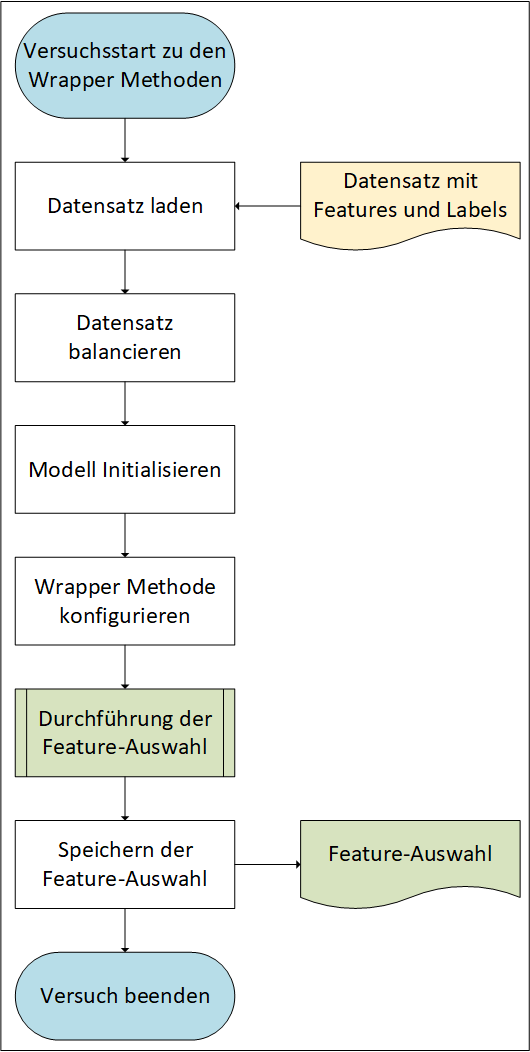
\includegraphics[height=0.9\textheight]{img/Grafiken/Flussdaigramm Versuche Wrapper Methoden.png}
    \caption{Flussdiagramm des Programmablaufs der Anwendung der Wrapper Methoden.}
    \label{fig:FlussDia Wrapper}
\end{figure}

Grundaufbau für die Versuche ist, dass der Feature-Datensatz, bestehend aus allen Feature-Kategorien, balanciert wird. Anschließend wird die Wrapper Methode konfiguriert. Die Wrapper Methode erhält ein Modell des maschinellen Lernens, die Features und die Labels. Anschließend wird die Auswahl durchgeführt. Die ausgewählten Features werden für die Evaluation gespeichert. Das Flussdiagramm in der Abbildung \ref{fig:FlussDia Wrapper} zeigt diesen Grundaufbau. 

Der Trainingsdatensatz mit den Features und den Labels wird wieder mit Hilfe der Bibliothek \textit{pandas} geladen. Der Datensatz muss balanciert werden. Dazu wird die Bibliothek \textit{imblearn} verwendet. Diese ist speziell auf den Umgang mit unbalancierten Datensätzen ausgelegt und implementiert Methoden, um diese zu balancieren. Verwendet wird das Undersampling (\autoref{sec:Meth Datensatz}). Der Codeauszug \ref{lst:Wrapp UnderSamp} zeigt die Anwendung von \textit{imblearn}. Die Durchführung der Wrapper Methode ist in einer Funktion implementiert. Diese nimmt ein Modell, die Datenmatrix und den Labelvektor entgegen. 

\begin{pythoncode}{Balancieren der Daten mit Undersampling.}{lst:Wrapp UnderSamp}
#Anwenden der Wrapper Methode
def wrapper_methode(modell, X, y):

    #Balancieren der Daten durch Undersampling
    from imblearn.under_sampling import RandomUnderSampler

    #Konfiguration des Undersamplings
    rus = RandomUnderSampler(sampling_strategy='not minority', 
                             replacement=False)
    
    #Durchführend des Undersamplings
    X_resampled, y_resampled = rus.fit_resample(X, y)

\end{pythoncode}

Der balancierte Datensatz ist nun für die Wrapper Methode verwendbar. Die Bibliothek \textit{scikit-learn} implementiert die Wrapper Methoden unter dem Namen \textit{SequentialFeatureSelector}. Eingestellt werden kann die Richtung des Wrappers: vorwärts oder rückwärts. Auch ob die Auswahl anhand einer Performancemetrik erfolgt oder ob eine bestimmte Anzahl an Features auszuwählen ist, kann eingestellt werden. Diese Optionen sowie das Modell sind die Parameter, die für die Versuche variiert werden. Die Modelle werden alle weitestgehend unkonfiguriert gelassen. Die Einstellung erfolgt in der Hyperparametersuche. Der Codeauszug \ref{lst:Wrapp InitRF} zeigt die Initialisierung und Konfiguration eines Random Forest Modells für eine Klassifikationsaufgabe. Alle Modelle aus der Vorauswahl sind in der Bibliothek \textit{scikit-learn} implementiert. Das macht die Anwendung der Modelle besonders einfach, da die Syntax zu Anwendung weitgehend gleich bleibt. Lediglich die Hyperparameter unterscheiden sich. 

\begin{pythoncode}{Initialisierung und Konfiguration eines Random Forest Modells.}{lst:Wrapp InitRF}
#Modell Initialisieren und Einstellen
from sklearn.ensemble import RandomForestClassifier
rf_classifier = RandomForestClassifier(n_estimators=100, 
                                       max_depth=5)
\end{pythoncode}

Im Codeauszug \ref{lst:Wrapp RUN} ist zu sehen, wie der Anwender die Einstellungen für die unterschiedlichen Versuche treffen kann. Damit wird die Wrapper Methode initialisiert und anschließend wird die Auswahl durchgeführt. Die Liste der Namen der ausgewählten Features wird für die Auswertung gespeichert. Für die Performance-Beurteilung soll die Metrik Accuracy verwendet werden.

\begin{pythoncode}{Konfigurieren und Anwenden der Wrapper Methode.}{lst:Wrapp RUN}
#verheriger Code innerhalb der Funktion Wrapper_methode...

#Wrapper Methode importieren
from sklearn.feature_selection import SequentialFeatureSelector

#Einstellungen für die Versuche
anzahl=50
#toleranz=0.001
richtung="forward" #"backward"

#Konfiguration der Wrapper Methode
wrapper = SequentialFeatureSelector(modell, 
                n_features_to_select=anzahl, 
                direction=richtung, 
                #tol=toleranz, 
                scoring="accuracy")

#Starten der Wrapper Methode
feat_auswahl = wrapper.fit_transform(X_resampled, y_resampled)
\end{pythoncode}



\subsection{Umsetzung der Hyperparametersuche}

\begin{figure}[p]
    \centering
    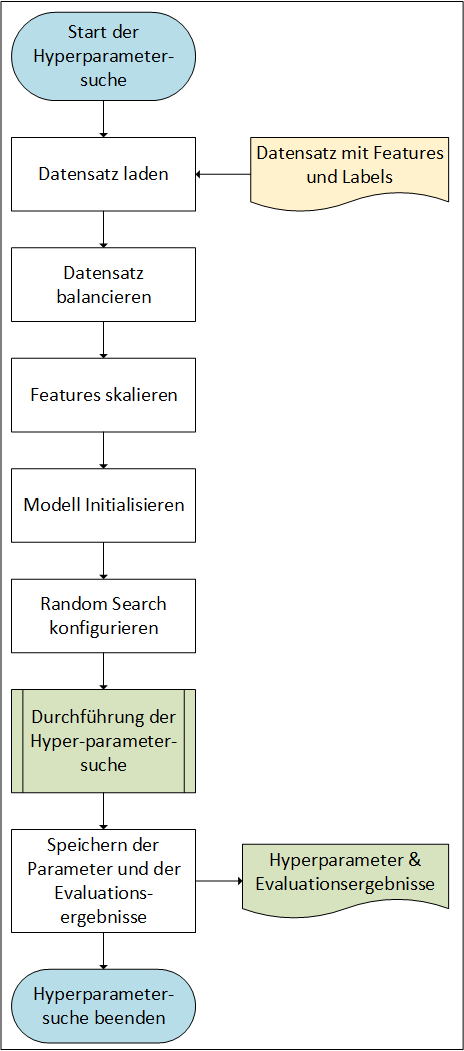
\includegraphics[height=0.9\textheight]{img/Grafiken/Flussdaigramm Hyperparametersuche.png}
    \caption{Flussdiagramm des Programmablaufs der Durchführung der Hyperparametersuche.}
    \label{fig:FlussDia Hyperpara}
\end{figure}

Die Hyperparametersuche erfolgt mittels einer Random Search. Diese ist für jedes Modell durchzuführen. Die Hyperparameter erhalten eine Verteilung zugewiesen, aus welcher die Random Search Werte zieht. Im Anhang befindet sich eine Darstellung der Hyperparameter der Modelle und wie sie für die Random Search konfiguriert werden. Im Folgenden wird die Durchführung beschrieben.  \par

Der Trainingsdatensatz wird geladen. Für die SVM müssen die Features skaliert werden. Anschließend wird der Datensatz balanciert. Die Hyperparameter bekommen ihre Verteilungen zugewiesen und die Random Search wird konfiguriert. Danach wird die Suche durchgeführt. Die gefundenen Parameter sowie die Validierungsergebnisse werden für die Auswertung abgespeichert. Dieser Ablauf ist im Flussdiagramm aus \autoref{fig:FlussDia Hyperpara} dargestellt.\par


Zunächst wird das Modell initialisiert. Das ist im Codeauszug \ref{lst:Hyp InitSVC} zu sehen. Hier wird eine SVM integriert, welche auf Klassifizierungsaufgabe ausgelegt ist. Im Vergleich zum Codeauszug \ref{lst:Wrapp InitRF}, in welchem ein Random Forest Model initialisiert wird, sind die Parallelen in der Syntax zu erkennen, um unterschiedliche Modelle zu verwenden. 

\begin{pythoncode}{Initialisieren der SVM für die Klassifikation.}{lst:Hyp InitSVC}
#Modell Initialisieren und Einstellen
#SVC - Support Vector Classification
from sklearn.svm import SVC
svm_classifier = SVC(kernel='poly')
\end{pythoncode}

Wie in \autoref{sec:Meth FeatVorSele} erwähnt, sind die Features auf den Wertebereich [-1; 1] zu skalieren, damit die SVM sinnvoll trainiert wird. Auch hierfür bietet die \textit{scikit-learn} Bibliothek Funktionen. Im Codeauszug \ref{lst:Skale} ist zu sehen, dass mit der Klasse \textit{MinMaxScaler} eine Datenmatrix auf einen angegebenen Wertebereich skaliert werden kann.\par

Vorteilhaft an der Verwendung von \textit{MinMaxScaler} ist, dass sich das Objekt \textit{scaler} die Skalierungsinformationen merkt. Beim Aufruf von \textit{fit} bzw. \textit{fit\_transform} wird das Objekt \textit{scaler} trainiert. Es kann gespeichert werden und wird für die Verarbeitung der Features in der Anwendung eingesetzt. 

\begin{pythoncode}{Skalieren der Features auf den erforderlichen Wertebereich.}{lst:Skale}
#Skalieren der Features 
from sklearn.preprocessing import MinMaxScaler
scaler = MinMaxScaler(feature_range=(-1,1))
X_scaled = scaler.fit_transform(X_resampled)
\end{pythoncode}

Die Hyperparameter benötigen Verteilungen, aus denen die Random Search Werte ziehen kann. Die Bibliothek \textit{scipy} implementiert Verteilungsfunktionen, die sich dafür verwenden lassen. Der Codeauszug \ref{lst:Hyp SVM} zeigt die Angaben für die Hyperparameter der SVM. Im Anhang ist eine ausführlichere Beschreibung der Hyperparameter und der Einstellung zu finden.

\begin{pythoncode}{Angaben der Verteilungen für die Hyperparameter der SVM.}{lst:Hyp SVM}
#Scipy für die Verteilungen
from scipy import stats

#Angabe der Verteilungen für die einzelnen Hyperparameter
hyperparams =  {"degree": [2, 3, 4, 5, 6],
                "coef0": stats.loguniform(1e-1, 1e3),
                "tol": stats.loguniform(1e-3, 1e0),
                "C": stats.loguniform(1e-1, 1e3),
                "decision_function_shape": ["ovo", "ovr"]}
\end{pythoncode}

Die Random Search ist ebenfalls in \textit{scikit-learn} implementiert. Diese muss vor der Durchführung eingestellt werden. Wie in \autoref{sec:Meth HyperparaKonf} beschrieben, werden 500 Kombinationen von Hyperparametern überprüft und jede Kombination wird 150-mal validiert. Das übliche Verfahren der Cross-Validation teilt den Trainingsdatensatz in feste Teile, die dann nacheinander für die Validierung eines Modells verwendet werden. Da die Menge an Validierungsdaten sehr klein wäre, wenn der Trainingsdatensatz in 150 Teile gesplittet wird, wird im Codeauszug \ref{lst:HypSerachRUN} die Klasse \textit{RepeatedKFold} verwendet. Über diese Klasse ist die Cross-Validation konfigurierbar. Sie implementiert ein Verfahren, bei welchem mehrere Wiederholungen der Zerteilung durchgeführt werden. Bei jeder Wiederholung wird der Trainingsdatensatz in zufällige, neue Teile gesplittet. Im Codeauszug \ref{lst:HypSerachRUN} wird Cross-Validation so konfiguriert, dass der Trainingsdatensatz in 10 Teile zerteilt wird. Mit dieser Aufteilung findet die klassische Cross-Validation statt. Anschließend wird der Trainingsdatensatz in 10 neue Teile gesplittet. Dies wird insgesamt 15-mal wiederholt, sodass final 150 Validierungsergebnisse pro Kombination vorhanden sind. \par

Die Random Search wird über die Klasse \textit{RandomizedSearchCV} konfiguriert. Sie bekommt die Einstellungen der Hyperparameter und der Cross-Validation übergeben. Auch die Anzahl der Ziehungen, das Modell und die Performance-Metrik werden eingestellt. Anschließend erfolgt die Durchführung über den Aufruf der Methode \textit{fit}. Die Ergebnisse werden zur Auswertung abgespeichert.

\begin{pythoncode}{Konfigurieren und Anwenden der Wrapper Methode.}{lst:HypSerachRUN}
#Importieren der Random Search und der Cross-Validation
from sklearn.model_selection import RepeatedKFold, RandomizedSearchCV

#Anzahl der Kombinationen, die gezogen werden sollen
n_iter = 500

#Einstellung der Cross-Validation
cross_vali = RepeatedKFold(n_splits=10, n_repeats=15)

#Konfigurieren der Random Search 
random_search = RandomizedSearchCV(svm_classifier, 
                                   hyperparams, 
                                   scoring="accuracy", 
                                   n_iter=n_iter, 
                                   cv=cross_vali)

random_search.fit(X_scaled, y_resampled)
\end{pythoncode}



\subsection{Trainieren und Testen des Models} 
Mit den gefundenen Hyperparametern sind nun die Modelle zu konfigurieren. Der Codeauszug \ref{lst:InitLogi} zeigt die Initialisierung einer logistischen Regression mit den gefundenen Hyperparametern. Wieder ist die Ähnlichkeit in der Syntax zur Initialisierung des Random Forest Modells und der SVM zu sehen. In der Random Search wurde eine L1 Regularisierung mit einem Faktor C von 5,75 als optimal gefunden. Der Parameter 'tol' ist ein Stop-Kriterium für die Lösung des Optimierungsproblems. Bezogen auf das Gradientenverfahren würde das Training frühzeitig beendet werden, wenn sich das Minimum bei einer Iteration nicht weiter als 0.0025 verbessert. 

\begin{pythoncode}{Einstellung der logistischen Regression mit den gefundenen Hyperparametern.}{lst:InitLogi}
#Modell Initialisieren mit gefundenen Parametern
from sklearn.linear_model import LogisticRegression
logiReg_classifier = LogisticRegression(C=5.75,
                                        fit_intercept=False,
                                        penalty='l1',
                                        tol=0.0025)
\end{pythoncode}

Noch vor der Feature-Vorauswahl und der Hyperparametersuche ist der Code aus dem Auszug \ref{lst:trainTest} auszuführen. In diesem wird der Datensatz aufgeteilt in Trainingsdatensatz und Testdatensatz. In der Umsetzung werden 20 \% der Daten für das Training beiseite gelegt. 

\begin{pythoncode}{Aufteilen des Datensatzes in Trainingsdaten und Testdaten.}{lst:trainTest}
#Daten in Trainings- und Testdatensatz teilen 
from sklearn.model_selection import train_test_split
X_train, X_test, y_train, y_test = train_test_split(X_resampled, y_resampled, test_size=0.2)
\end{pythoncode}

Abschließend wird das Modell mit dem Befehl \textit{fit} und den Trainingsdaten trainiert. Die Methode \textit{score} ermittelt die Accuracy mittels der Testdaten. Das ist im Codeauszug \ref{lst:TrainTestModelle} zu sehen. 

\begin{pythoncode}{Trainieren und Testen des fertigen Modells.}{lst:TrainTestModelle}
#Modelltraining und abschließende Evaluation
logiReg_classifier.fit(X_train, y_train)
test_score = logiReg_classifier.score(X_test, y_test)
\end{pythoncode}